\chapter{Validation}

\minitoc

\section{Beam systems}
\section{Validation}
\label{sec:valid}
In this section numerical simulations are performed to assess the correctness of the proposed formulation. {The examples make use of Euler Bernoulli beam model \eqref{eq:EB_sys}. To discretize the system, Lagrange polynomial of order one and Hermite polynomials of order 3 are used for $v_f^x$ and $v_f^y$ respectively. Discontinuous Galerkin elements of order 0 and 1 are selected for $n_x$ and $m_{x}$ respectively. This choice ensures the conformity with respect to the differential operator. As a first example the vertical vibrations of a simply supported beam are considered. To assess the validity of the finite elements, a convergence study with respect to an analytical solution is performed}. A {second} example concerns the computation of eigenvalues of a four bar {mechanism} for different geometrical configuration. The {third} example is a rotating crank-slider. In this case the non-linearities cannot be neglected. The {fourth} example is a hinged beam undergoing external excitations so that the out-of-plane motion becomes important.  The Firedrake python library \cite{rathgeber2017firedrake} is employed to construct the finite-dimensional discretization.  


\subsection{Linear analysis of a four-bar mechanism}

\begin{figure}[tb]
	\centering
	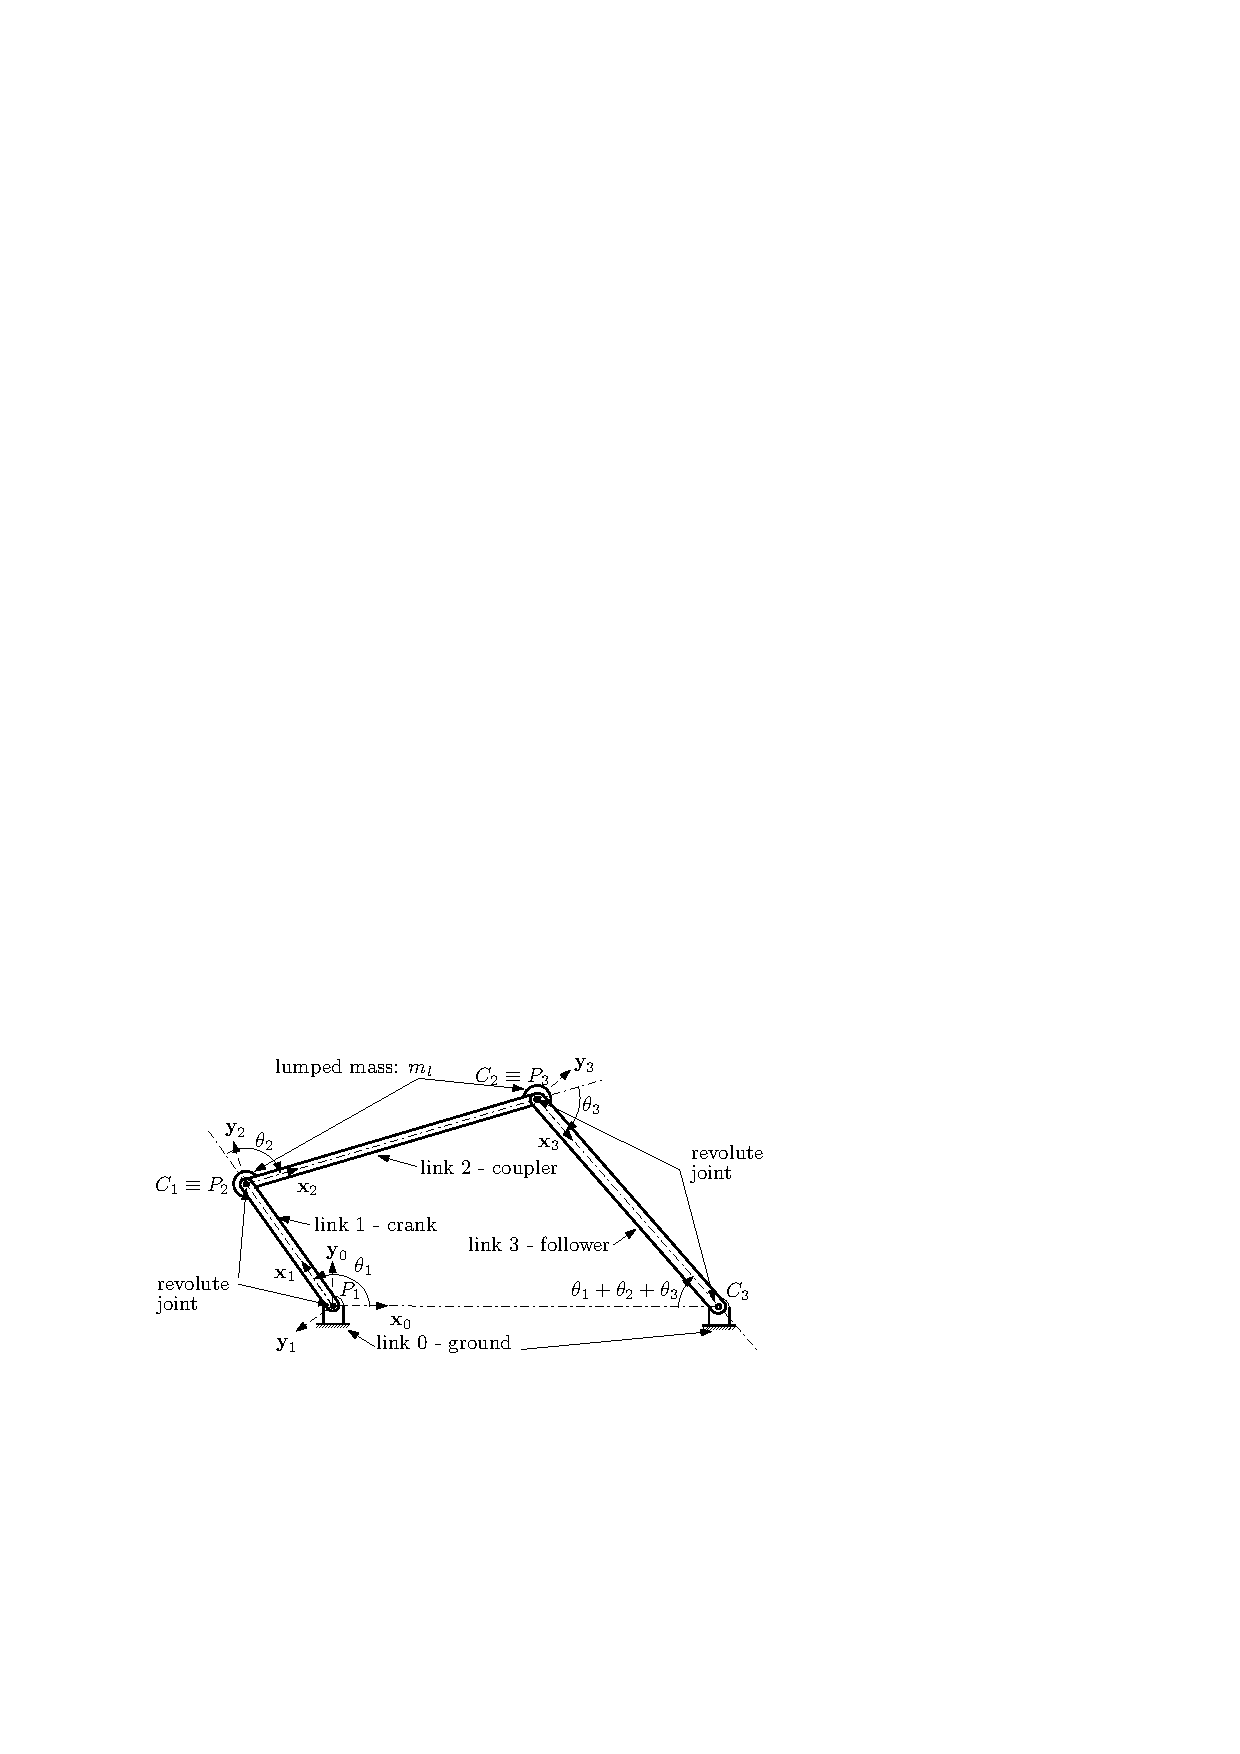
\includegraphics[width=0.6\textwidth]{part_4/validation/fourbars.pdf} 
	\includegraphics[width=0.35\textwidth]{part_4/validation/block_4bars.eps} 
	\caption{Four bar mechanism illustration (left) and block diagram used for the eigenvalues analysis (right)}
	\label{fig:4bars}
\end{figure}

\begin{table}[bt]
	% table caption is above the table
	\caption{Four-bar mechanism links properties: each link is a uniform beam with mass density $\rho=2714\,[\mathrm{kg}/\mathrm{m}^3]$ and Young modulus $E=7.1\,10^{10}\,[\mathrm{N}/\mathrm{m}^2]$. }
	\label{tab:data_4bars}       % Give a unique label
	% For LaTeX tables use
	\begin{tabular}{lllll}
		\hline\noalign{\smallskip}
		$i$ & $0$ &  $1$ &  $2$ &  $3$  \\
		\noalign{\smallskip}\hline\noalign{\smallskip}
		Name & ground & crank & coupler & follower \\ 
		Length $L_i\,[\mathrm{m}]$ & $0.254$ & $0.108$ & $0.2794$ & $0.2705$\\
		Cross section $A_i\,[\mathrm{m}^2]$ & $-$ & $1.0774\,10^{-4}$ & $4.0645\,10^{-5}$ & $4.0645\,10^{-5}$ \\
		Flexural rigidity $(EI)_i\,[\mathrm{Nm}^2]$ & $-$ & $11.472$ & $0.616$ & $0.616$ \\
		\hline
	\end{tabular}
\end{table}

The four-bar mechanism has one degree of freedom and represents a closed chain of bodies. The data are taken from \cite{kitis1990natural,chebbi2017} are recalled in Table \ref{tab:data_4bars}. In Fig. \ref{fig:4bars} the mechanism and the corresponding block diagram used for constructing the final pH system with transformer interconnections between subsystems are presented. The lumped masses are directly included in the coupler and follower model considering a simple modification of the rigid mass matrix
\begin{equation*}
\mathbf{M}_{rr}^{i + m_l}[1:2,1:2] = \mathbf{M}_{rr}^{i}[1:2,1:2] + \mathbf{I}_{2\times 2} m_l,
\end{equation*} 
where $i=2,3$ denotes the coupler or follower model. Given a certain crank angle $\theta_1$ the relative angles between the different links are found by solving the two kinematic constraints
\begin{align*}
L_1 \cos(\theta_1)+ L_2 \cos(\theta_1+\theta_2)+ L_3 \cos(\theta_1+\theta_2+\theta_3) &=L_0, \\
L_1 \sin(\theta_1)+L_2 \sin(\theta_1+\theta_2)+L_3 \sin(\theta_1+\theta_2+\theta_3) &=0.
\end{align*} 
Once the angles describing the geometrical configuration are known, the transformer interconnection \eqref{eq:int_hinge} is applied to insert a revolute joint between adjacent links. For the deformation field a cantilever condition is imposed for each beam. The resulting system is then constrained to ground by imposing to following equalities
\begin{equation*}
\mathbf{v}_{P_1} = 0, \quad \omega^z_{P_1} = 0, \quad \mathbf{v}_{C_3} = 0.
\end{equation*}
The resulting system is expressed in pH form as $\mathbf{E}\dot{\mathbf{e}} = \mathbf{J} \mathbf{e}$. The eigenfrequencies are then found by solving the generalized eigenvalue problem $\mathbf{E}\bm{\Phi} = \mathbf{J} \bm{\Phi \Lambda}$. Since $\mathbf{J}$ is skew-symmetric the eigenvalues will be imaginary $\bm{\Lambda} = j \bm{\Omega}$. The first three pulsations  are reported in Fig. \ref{fig:omega_4bars} for different values of the crank angle $\theta_1$. The results match those of \cite{chebbi2017} (labeled as TITOP in the figure), assessing the validity of the linear model.

\begin{figure}[tb]
	\centering
	\includegraphics[width=0.49\textwidth]{part_4/validation/FourBar_Om12_Chebbi.eps} 
	\includegraphics[width=0.49\textwidth]{part_4/validation/FourBar_Om3_Chebbi.eps} 
	\caption{Eigenvalues $\omega_i, \ i=1,2,3$ for the four bar mechanism for varying crank angle.}
	\label{fig:omega_4bars}
\end{figure}

\subsection{Rotating crank-slider}
To verify the non-linear planar model a crank-slider rotating at high speed is considered. The example is retrieved form \cite{ellenbroek2018}.  The crank is considered as rigid, with length $L_{\text{cr}} = 0.15 \ [\mathrm{m}]$ and rotates at a constant angular rate $\omega_{\text{cr}} = 150 \ [\mathrm{rad/s}]$. The flexible coupler has length $L_{\text{cl}} = 0.3 \ [\mathrm{m}]$ and a circular cross section whose diameter is $d_{\text{cl}} = 6 \ [\mathrm{mm}]$. Its Young modulus and density are given by $E_{\text{cl}}=0.2 \ 10^{12} \ [\mathrm{Pa}]$, and $\rho_{\text{cl}}=7870 \ [\mathrm{kg/m}^3]$. The slider has a total mass equal to half the mass of the coupler $m_{\text{sl}} = 0.033 \ [\mathrm{kg}]$. A simply supported condition is supposed for the coupler deformation field. This choice is motivated by the fact that the slider has a large inertia and does not allow elastic displacement at the tip.

\begin{figure}[tb]
	\centering
	\includegraphics[width=0.5\textwidth]{part_4/validation/cr_slider.eps} 
	\includegraphics[width=0.4\textwidth]{part_4/validation/block_crslider.eps} 
	\caption{Crank slider illustration (left) and block diagram (right)}
	\label{fig:crsl}
\end{figure}

An illustration of the system and the block diagram used to construct the model are provided in Fig. \ref{fig:crsl}. To construct the crank slider a transfomer interconnection is first used to connect the slider to the flexible coupler. The motion of the slider is then computed in the coupler reference frame. Then the sliding constraint, that requires the vertical velocity of the slider to be null in the inertial frame, is imposed as follows
\[
0 = \sin(\theta_{P_1}) v^x_{P_2} + \cos(\theta_{P_1}) v^y_{P_2} = \mathbf{R}_y(\theta_{P_1}) \mathbf{v}_{P_2},
\]
where $\mathbf{R}_y$ is the second line of the rotation matrix and ${\theta}_{P_1}$ is the angle defining the orientation of the coupler. The rigid crank velocity at the endpoint  
\begin{equation*}
\mathbf{v}_{\text{cr}}(t) = -\omega_{\text{cr}} L _{\text{cr}} \sin(\omega_{\text{cr}} t) \widehat{\mathbf{X}} + \omega_{\text{cr}} L _{\text{cr}} \cos(\omega_{\text{cr}} t) \widehat{\mathbf{Y}}
\end{equation*} 
has to be written in the coupler reference frame to get the input
\begin{equation*}
\mathbf{u}_{\text{cl}} = R(\theta_{P_1})^\top \mathbf{v}_{\text{cr}}.
\end{equation*}
The resulting system is a quasi linear index-2 DAE of the form
\begin{equation*}
\begin{bmatrix}
\mathbf{M} & 0 & 0 \\
0 & 0 & 0 \\
0 & 0 & 0 \\
\end{bmatrix}
\begin{bmatrix}
\dot{\mathbf{e}} \\ \dot{\bm{\lambda}}_0 \\ \dot{\bm{\lambda}}_u \\
\end{bmatrix}= 
\begin{bmatrix}
\mathbf{J}(\mathbf{e}) & \mathbf{G}_0^\top(\theta_{P_1}) & \mathbf{G}_u^\top \\
-\mathbf{G}_0(\theta_{P_1}) & 0 & 0 \\
-\mathbf{G}_u & 0 & 0 \\
\end{bmatrix}
\begin{bmatrix}
\mathbf{e} \\ \bm{\lambda}_0 \\ \bm{\lambda}_u \\
\end{bmatrix} + 
\begin{bmatrix}
0 \\ 0 \\ R(\theta_{P_1})^\top \\
\end{bmatrix}
\mathbf{v}_{\text{cr}}.
\end{equation*}


\begin{figure}[tb]
	\centering
	\includegraphics[width=0.45\textwidth]{part_4/validation/uM_disp.eps} 
	\includegraphics[width=0.45\textwidth]{part_4/validation/wM_disp.eps} 
	\caption{Coupler midpoint horizontal (left) and vertical (right) displacement}
	\label{fig:defM_crsl}
\end{figure}

Setting the initial conditions properly is of utmost  importance for a DAE solver. For this problem the beam is supposed undeformed at the initial time. The initial conditions for the rigid movement are then found using basic kinematics considerations.  The system is then solved using the IDA algorithm available in the Assimulo library \cite{assimulo2015}. The computational performance for this test case are reported in Tab. \ref{tab:comp_perf_crslider} In Fig. \ref{fig:defM_crsl} the midpoint deformation displacement $u_f^x(L_{\text{cl}/2}),\; u_f^y(L_{\text{cl}/2})$, normalized with respect to the coupler length, is reported. The resulting vertical displacement is in accordance with the results presented in \cite{ellenbroek2018}. The horizontal displacement exhibits high oscillations because of the higher eigenfrequencies of the longitudinal movement. This is due to the fact that null initial conditions are imposed on the deformation \cite{simeon2006}. In order to obtain a smoother solution, the initial deformation has to be computed from the rigid initial condition.


\begin{table}[tb]
	\centering
	% table caption is above the table
	\caption{{Computational performances for the crank slider.}}
	\label{tab:comp_perf_crslider}       % Give a unique label
	% For LaTeX tables use
	\begin{tabular}{cccc}
		\hline\noalign{\smallskip}
		Solver & Elapsed simulation time & Average $\Delta t$ & Final time \\
		\noalign{\smallskip}\hline\noalign{\smallskip}
		IDA & $12.14\; \mathrm{[s]}$ & $4.98 \, 10^{-7} \; \mathrm{[s]}$ & $0.053 \, 10^{-4} \; \mathrm{[s]}$\\
		\hline
	\end{tabular}
\end{table}

\subsection{Hinged spatial beam}
A spatial beam rotating about a spherical joint is considered (see Fig. \ref{fig:beam_3D}). This example was considered in \cite{cardona2000,ellenbroek2018}. The physical parameters are briefly recalled in Table \ref{tab:data_3Dbeam}. The spherical joint constraint is imposed by setting to zero the linear velocity, while a cantilever is imposed for the deformation field as the tip is free. For the first $10.2 [\mathrm{s}]$ a torque $ M_z =200 [\mathrm{N/mm}]$ is applied about the vertical axis. Then, an impulsive force $ F_z =100 [\mathrm{N}]$ is applied at the tip of the beam at $15 [\mathrm{s}]$, to excite the out-of-plane movement. The system is solved using an implicit Runge-Kutta method of the Radau IIA family {(see Tab. \ref{tab:comp_perf_hinged} for the computational performance of this test case)}. The simulation results, provided in Fig. \ref{fig:H_omega}, correspond to the total energy and the angular velocity measured in the inertial vertical direction. The result matches with the provided references. Indeed the non-linearities associated to the gyroscopic terms are small as the maximum angular velocity is equal to $0.1 \ [\mathrm{rad/s}] \approx 5 \ [\mathrm{deg/s}]$. 

\begin{figure}[tb]
	\centering
	\includegraphics[width=0.45\textwidth]{part_4/validation/rotbeam_3D.eps} 
	\caption{Spatial beam on a spherical joint.}
	\label{fig:beam_3D}
\end{figure}

\begin{figure}[tb]
	\centering
	\includegraphics[width=0.45\textwidth]{part_4/validation/H_3Dbeam.eps} 
	\includegraphics[width=0.45\textwidth]{part_4/validation/omega_zI.eps} 
	\caption{Simulation results: kinetic energy (left) and angular velocity about the vertical inertial direction (right).}
	\label{fig:H_omega}
\end{figure}

\begin{table}[tb]
	% table caption is above the table
	\caption{Physical parameters for the hinged spatial beam.}
	\label{tab:data_3Dbeam}       % Give a unique label
	% For LaTeX tables use
	\begin{tabular}{lllll}
		\hline\noalign{\smallskip}
		Length & Cross section & Inertia moment & Density & Young modulus \\
		\noalign{\smallskip}\hline\noalign{\smallskip}
		141.45 $[\mathrm{mm}]$ & 9.0 $[\mathrm{mm}^2]$ & 6.75 $[\mathrm{mm}^4]$ & 7800 $[\mathrm{kg/mm}^3]$ & 2.1 $10^6 \ [\mathrm{N/m}^2]$  \\
		\hline
	\end{tabular}
\end{table}


\begin{table}[tb]
	\centering
	% table caption is above the table
	\caption{Computational performances for the hinged spatial beam.}
	\label{tab:comp_perf_hinged}       % Give a unique label
	% For LaTeX tables use
	\begin{tabular}{cccc}
		\hline\noalign{\smallskip}
		Solver & Elapsed simulation time & Average $\Delta t$ &  Final time \\
		\noalign{\smallskip}\hline\noalign{\smallskip}
		Radau IIA & $21.14\; \mathrm{[s]}$ & $6 \; 10^{-4} \; \mathrm{[s]}$ & $50 \; \mathrm{[s]}$ \\
		\hline
	\end{tabular}
\end{table}


\section{Plate systems}
\subsection{Boundary interconnection with a rigid element}
\subsection{Actuated plate}



\section{Conclusion}


There are however many questions that require further investigations. To address complex multibody systems, higher dimensional models (plates, shells and 3D continua) have to be considered. Port-Hamiltonian plate models and 3D continua are readily available, whereas the reformulation of shell structures in pH form is still an open topic. For 3D continua and thick plate models (Mindlin-Reissner plates) one may employ the method proposed in \cite{cohen2005} to achieve the discretization. The discretization of thin plate models is substantially more difficult. \\ 
The employment of finite elements leads to large sparse systems to be solved. To limit the computational complexity of these models, model reduction techniques can be incorporated. While for linear pHDAE systems consolidated methodologies exist \cite{egger2018}, for the  non linear differential-algebraic case solutions are not yet available. To avoid the problem of dealing with large-scale systems, spectral methods can be equivalently used to achieve a structure preserving discretization made up of small and dense matrices.  \\ 
The time-domain simulations of the resulting systems have been accomplished using ready-to-use solvers. A rigorous numerical analysis, out of the scope of this paper, represents an important future development. In particular, numerical methods capable of preserving important structural properties in discrete time have been studied for rigid body dynamics \cite{celledoni2018passivity} and generic ODE \cite{kotyczka2019discrete} and DAE \cite{mehrmann2019structurepreserving} pH systems. These methods could be fruitfully employed in the proposed framework. 